\chapter{System Description}

- System war schon durch vorheige Experimente weitgehend aufgebaut und besteht aus 3D gedruckten Teilen, einem Stepper Motor, Kamera, 2 metallischen Stangen, Zahnriemen und diversen mechanischen Teilen (siehe \ref{fig:overview_cart_pole_experiment})
\begin{figure}[htbp]
    \centering
    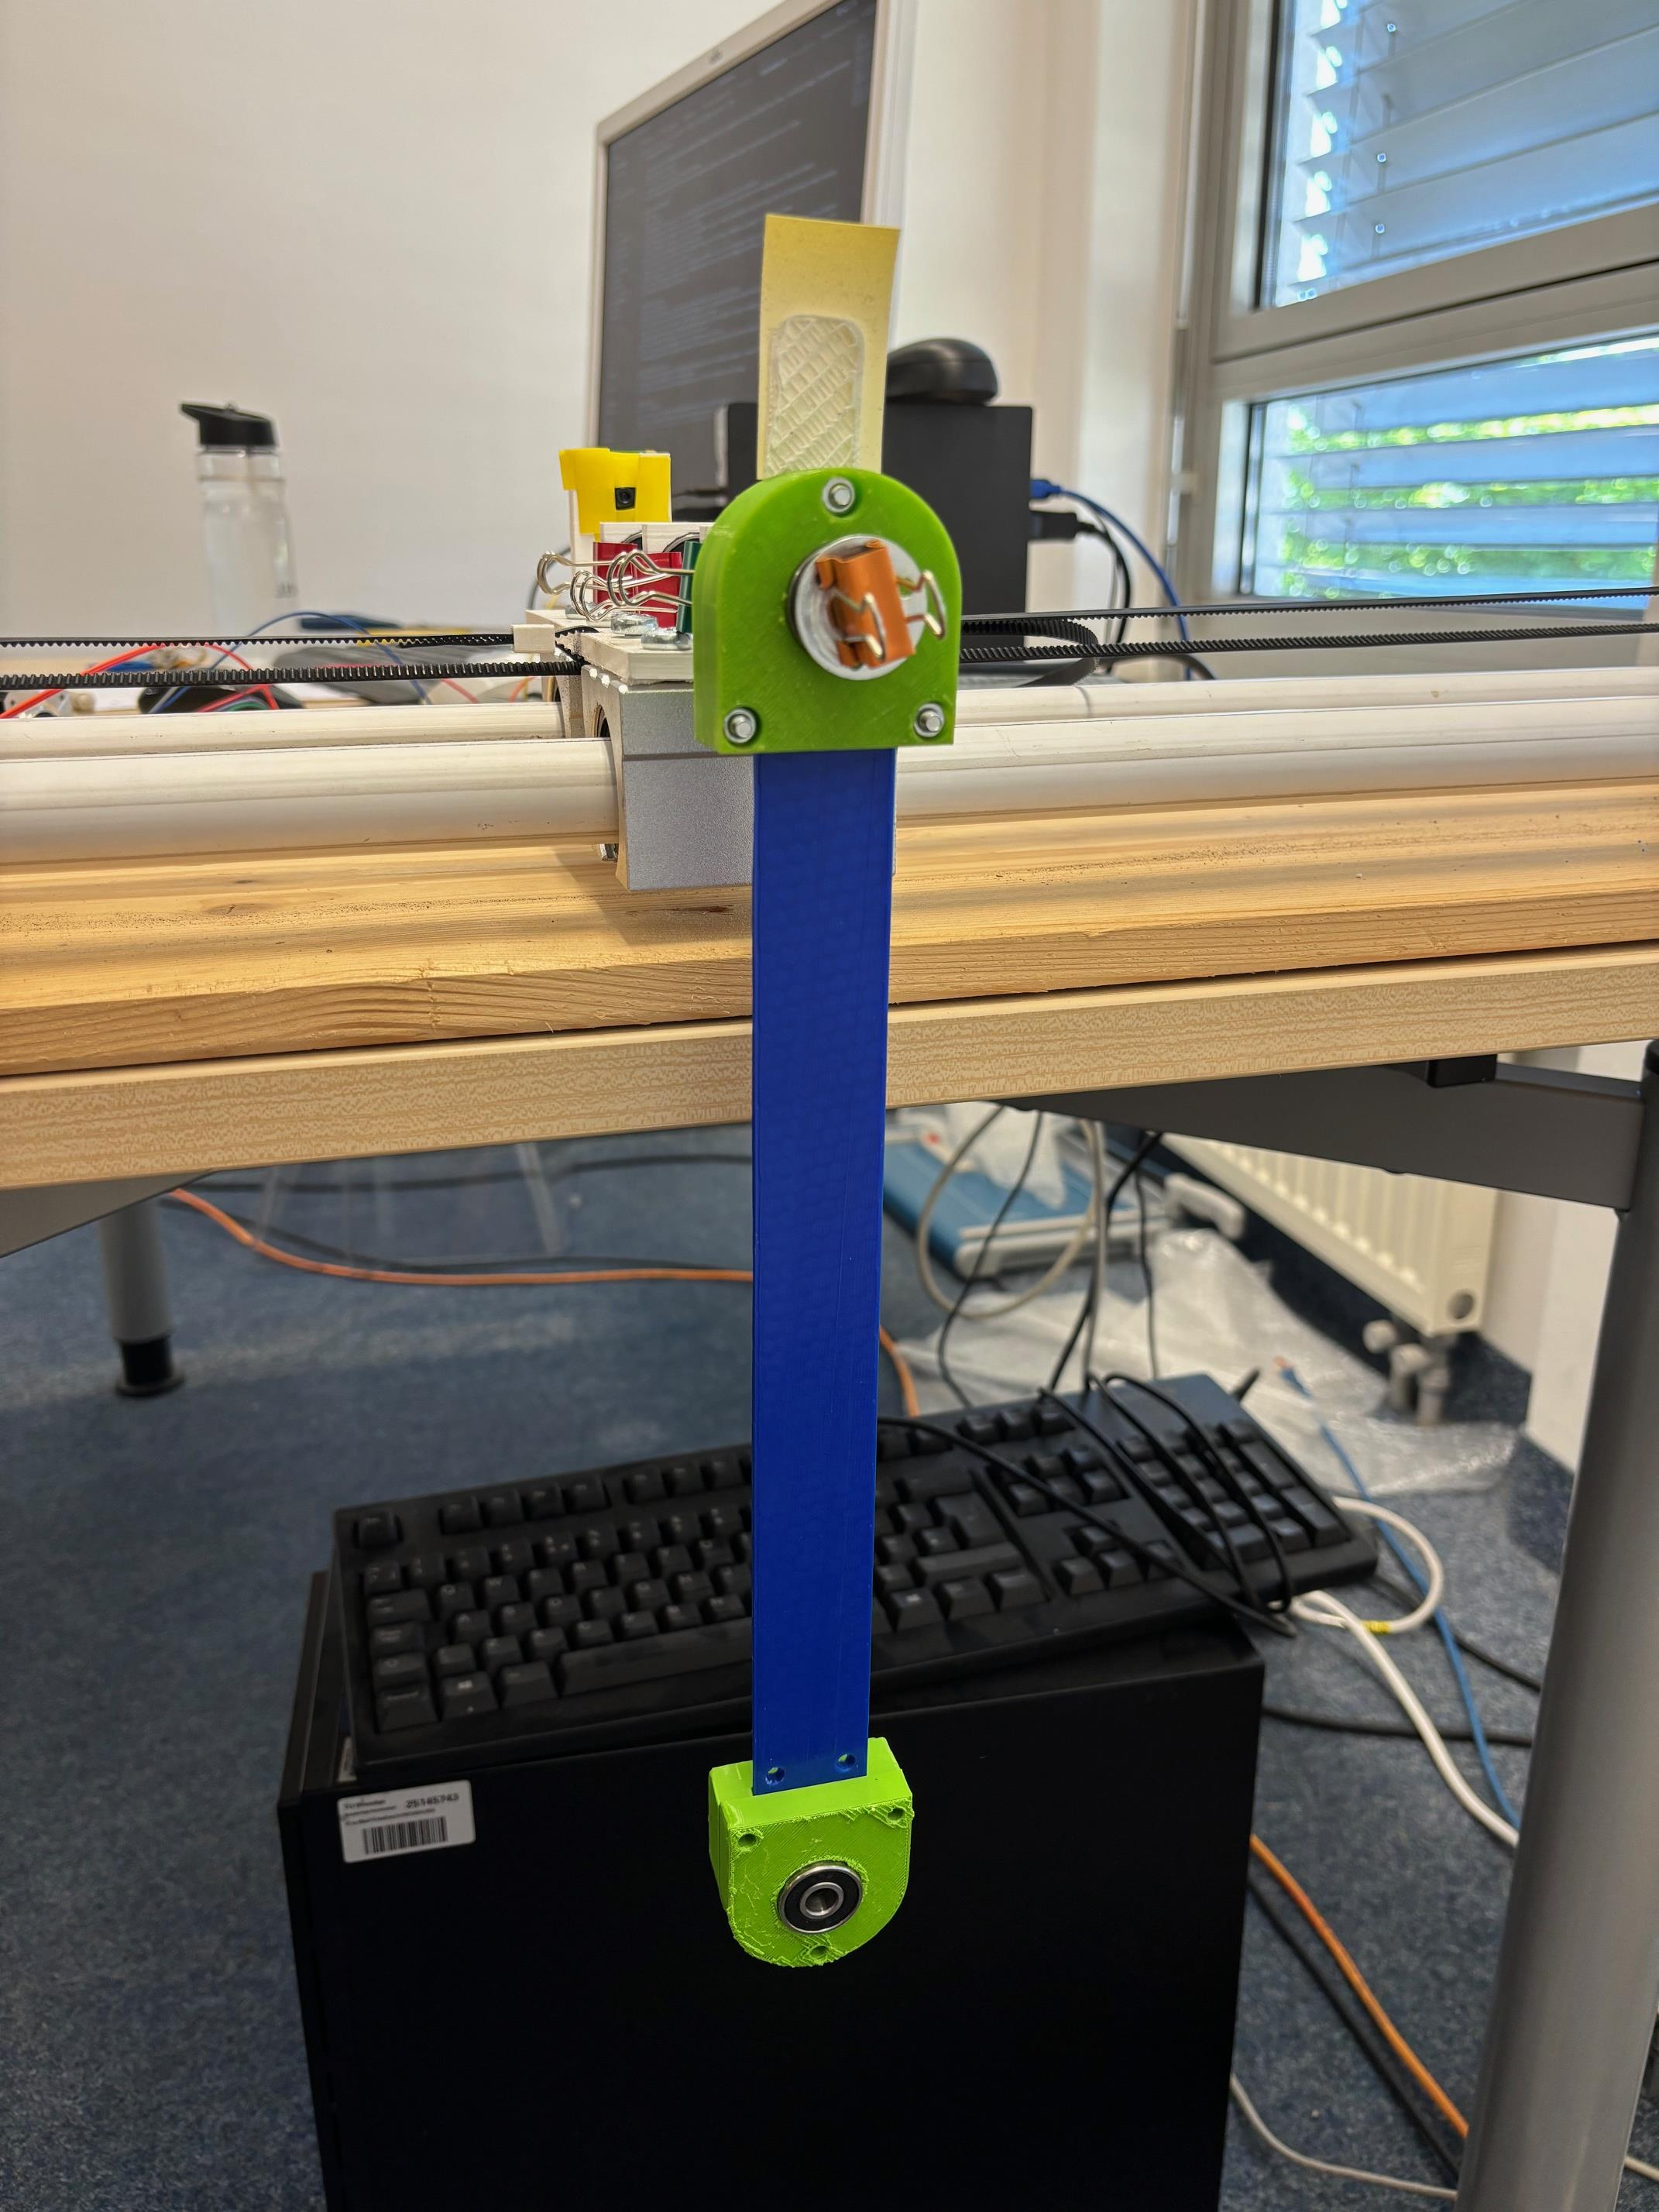
\includegraphics[width=0.4\textwidth]{img/front.jpg}
    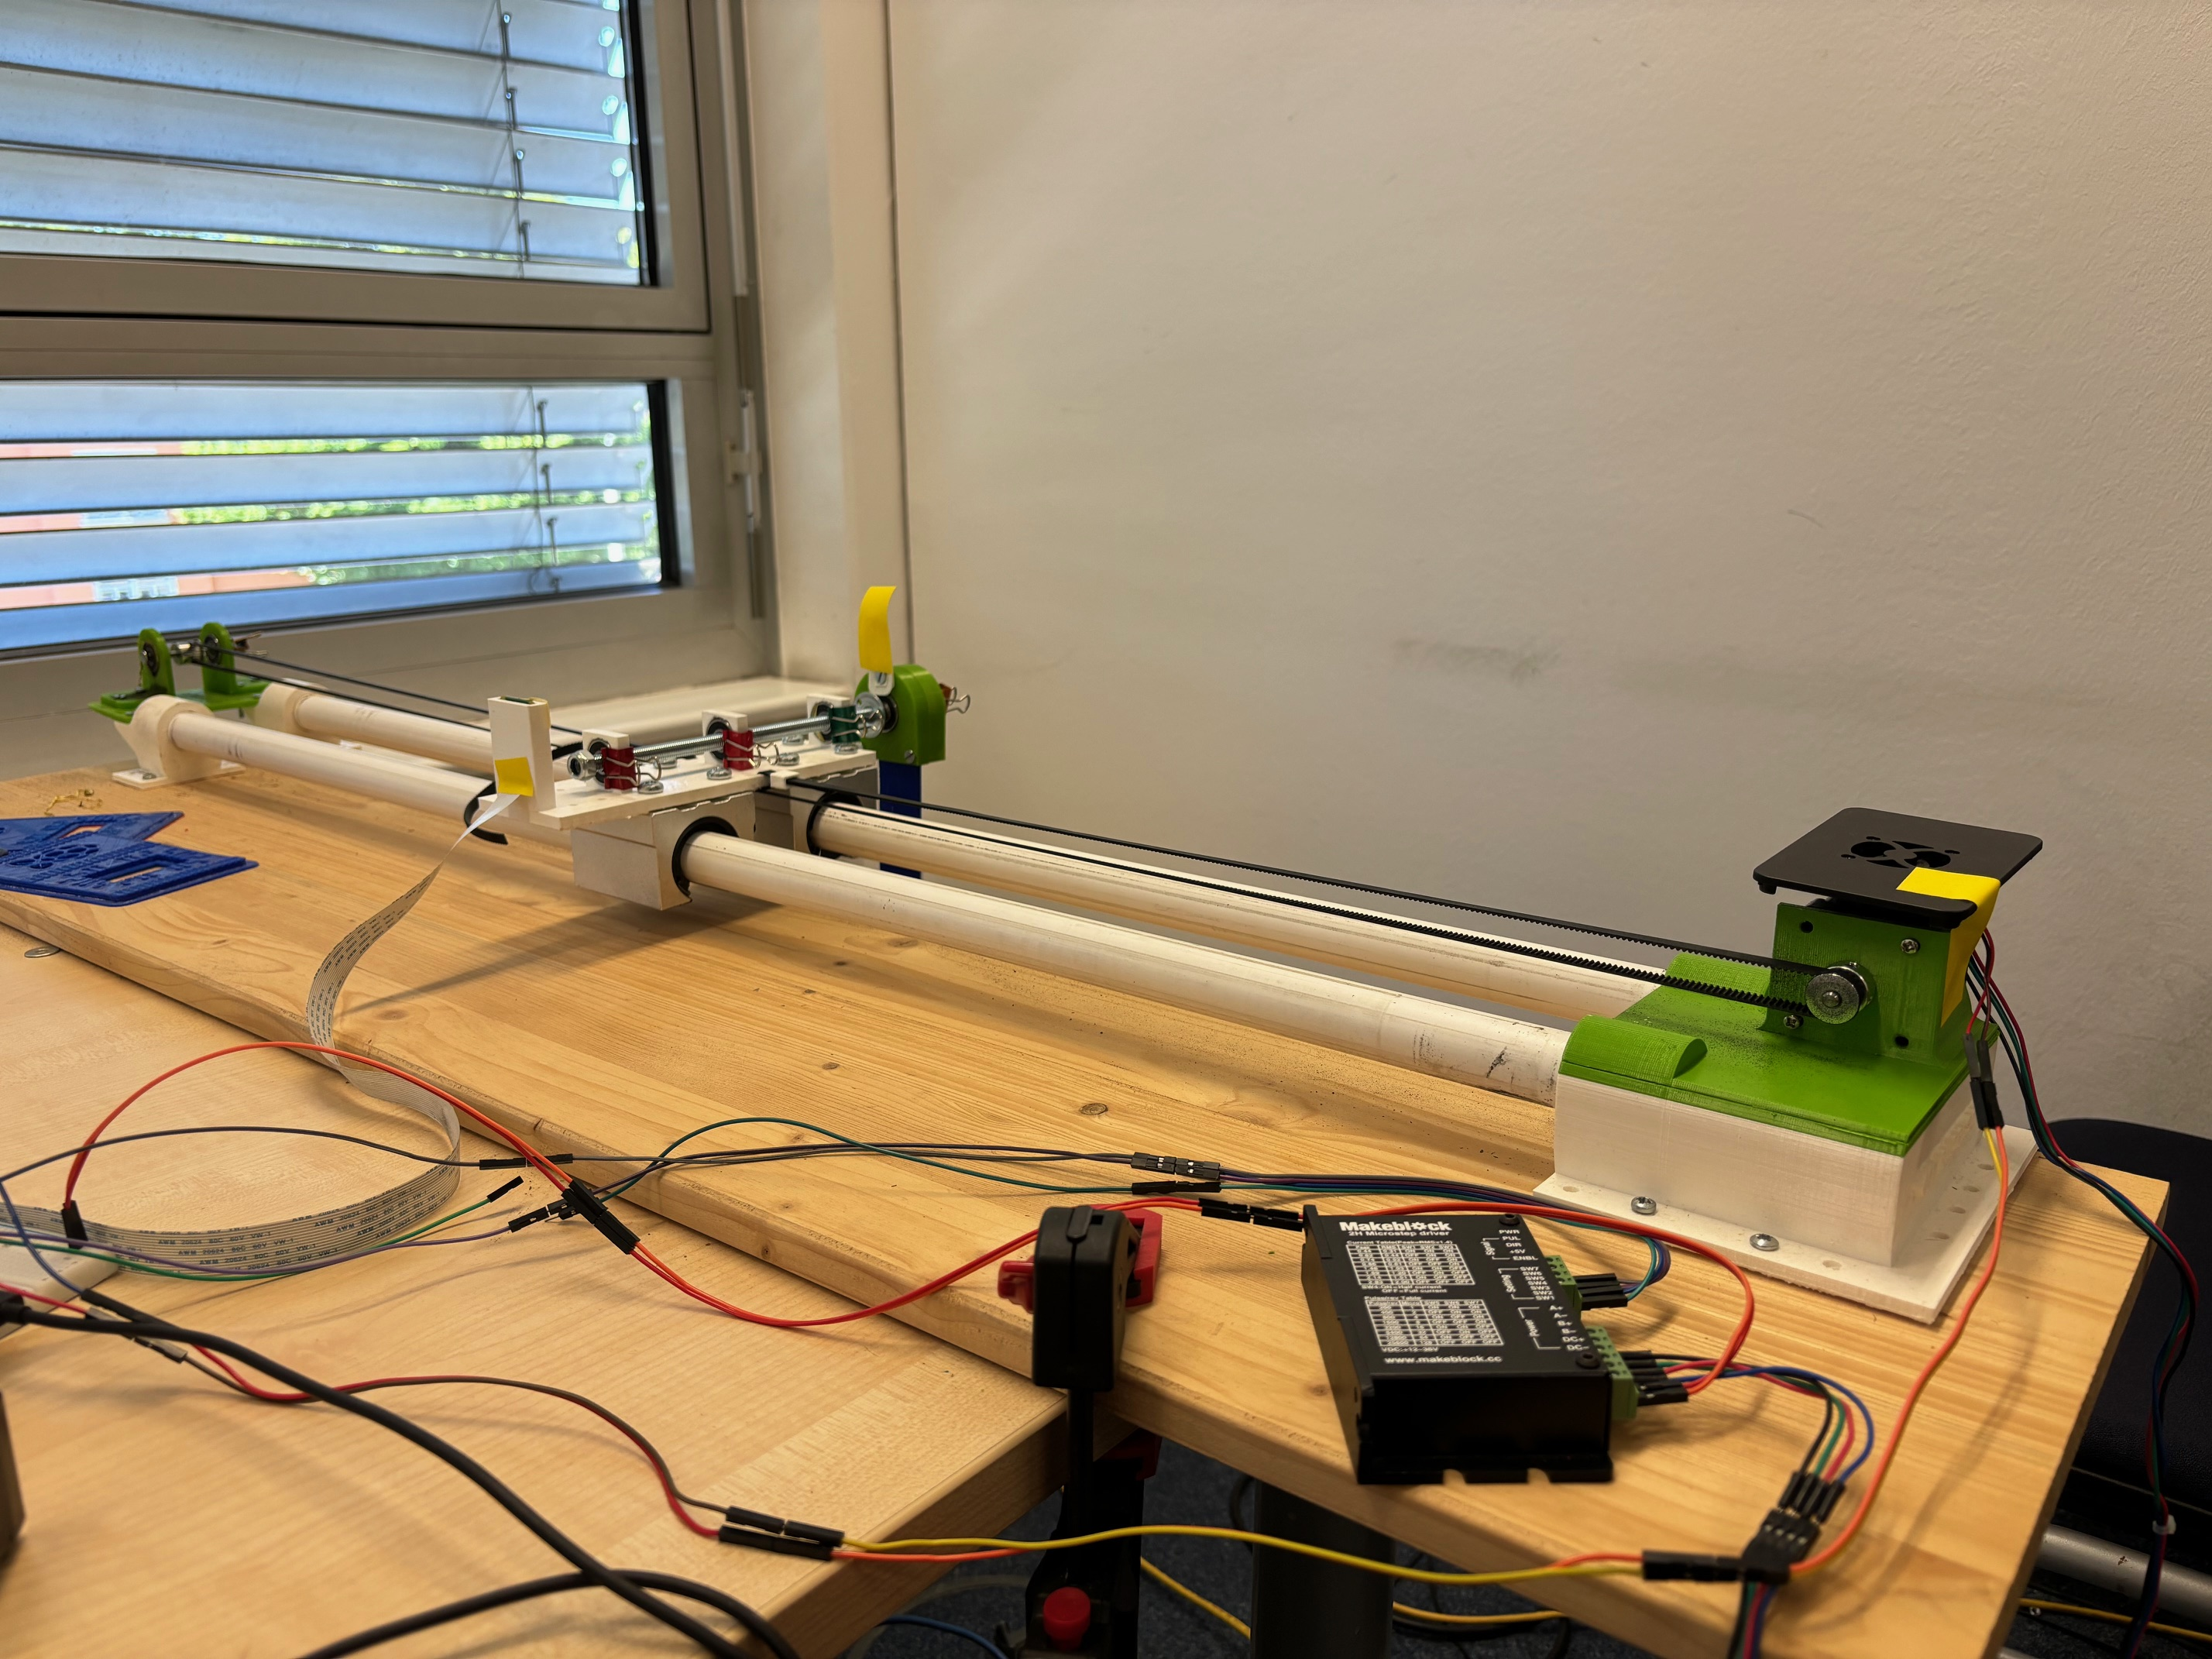
\includegraphics[width=0.4\textwidth]{img/back.jpg}
    \caption{Overview over Cart-Pole experiment with 3D printed parts}
    \label{fig:overview_cart_pole_experiment}
\end{figure}
- Anpassungen wurden im Verlauf der Experimente vorgenommen
- einige der beweglichen Teile haben sich im Laufe der Experimente verschoben, sodass Klammern angebracht werden mussten, um die Teile zu fixieren (\ref{fig:clamps})
\begin{figure}[htbp]
    \centering
    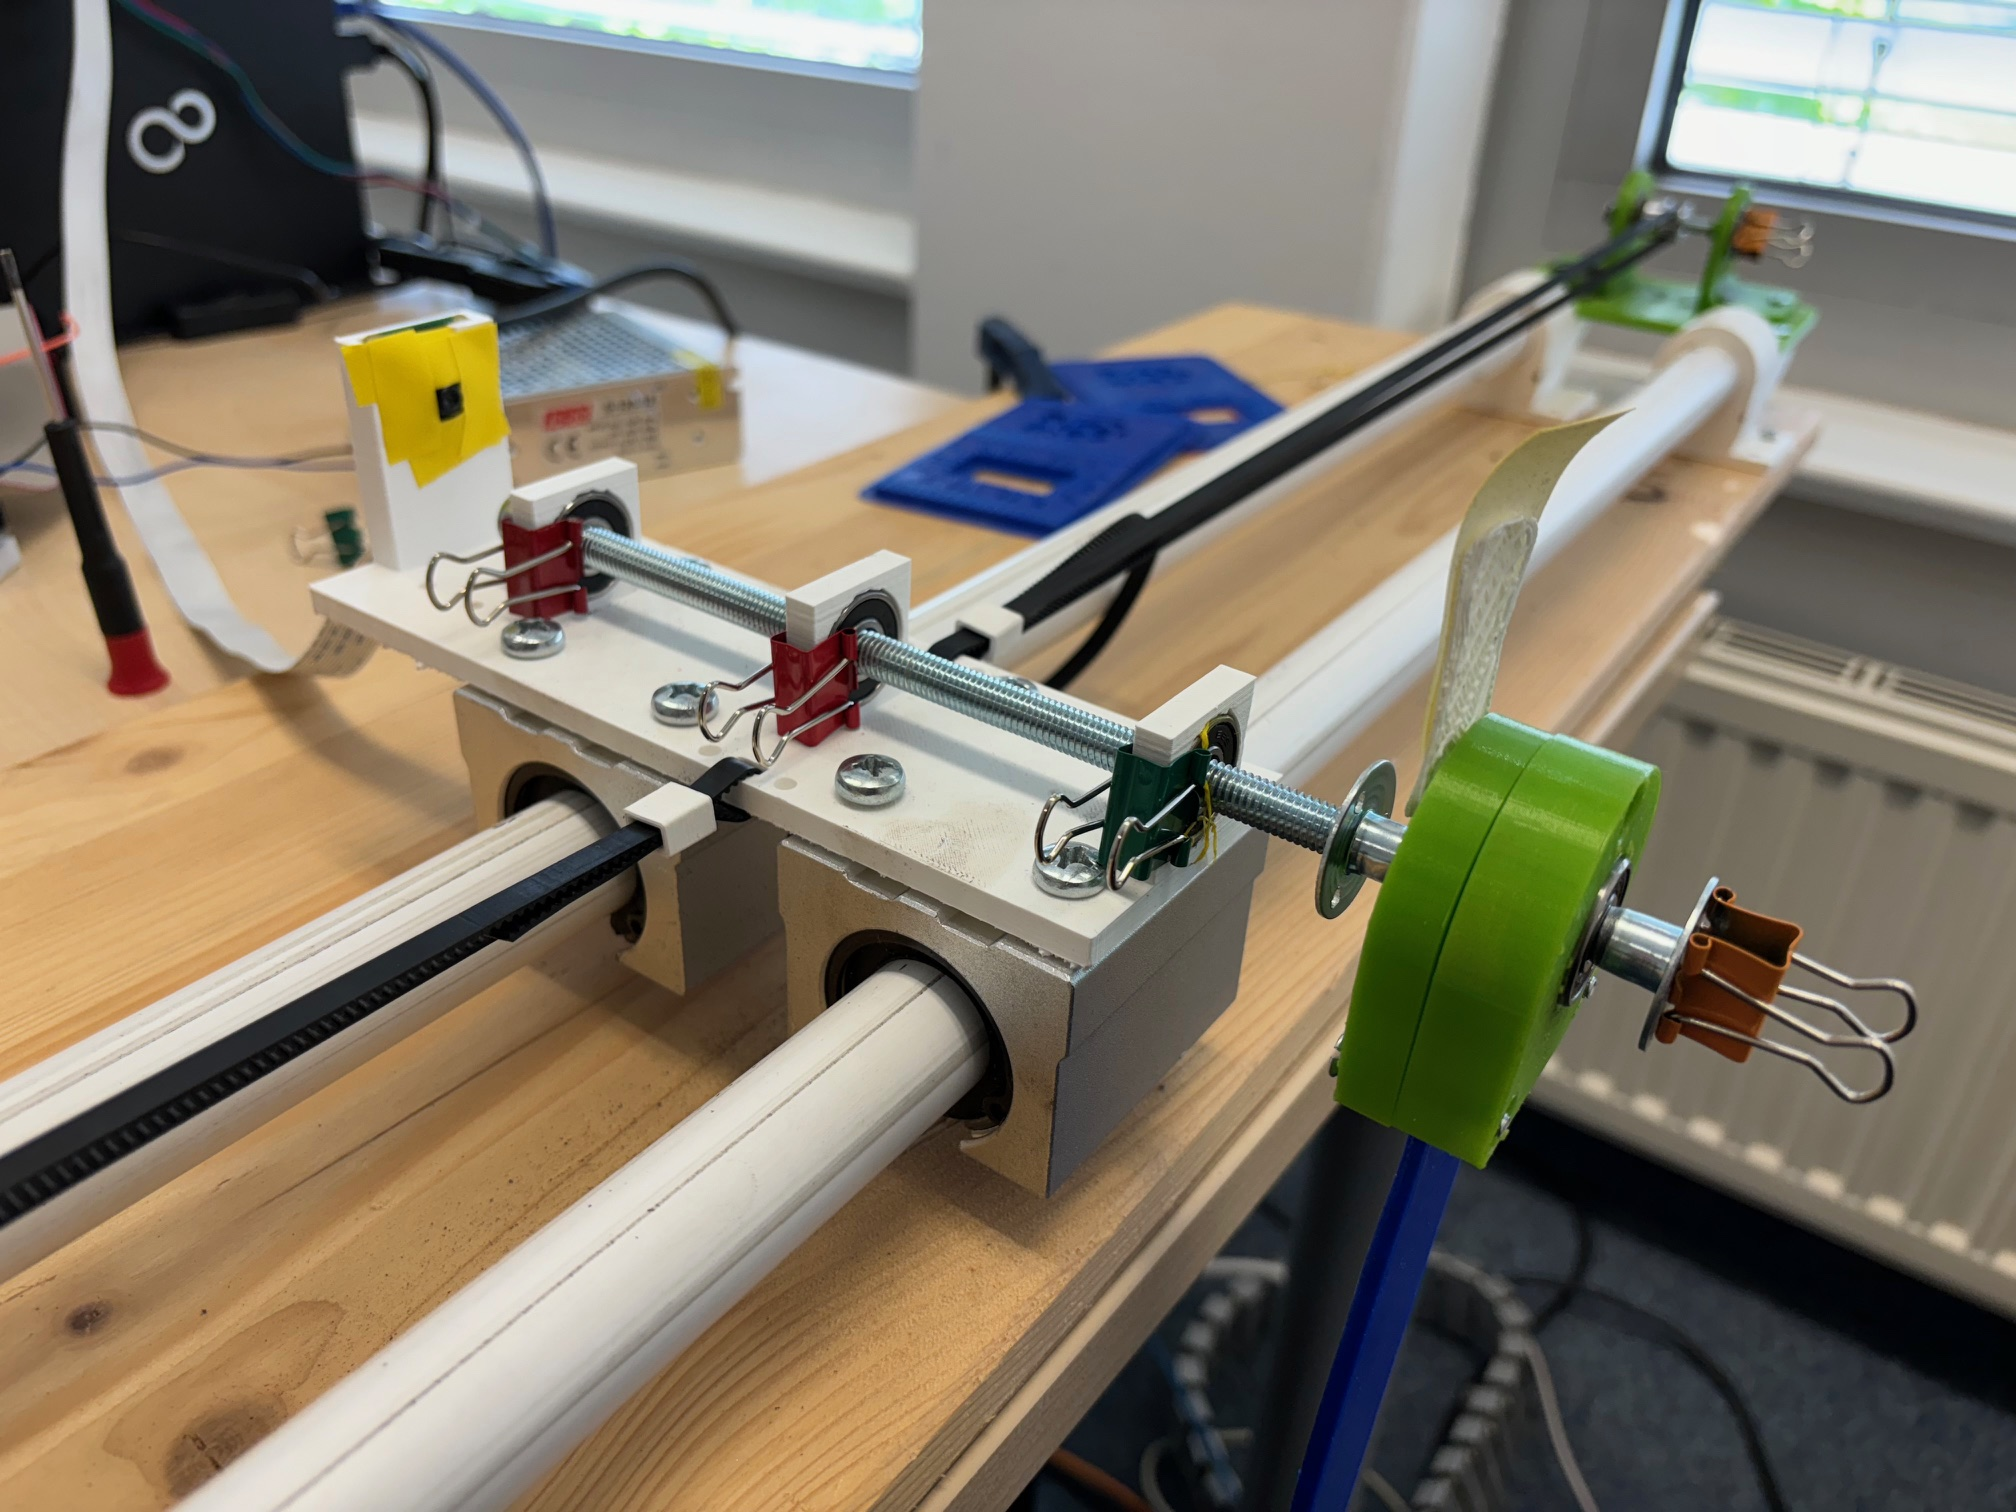
\includegraphics[width=0.8\textwidth]{img/clamps.jpg}
    \caption{Clamps to fixate moving parts}
    \label{fig:clamps}
\end{figure}

\section{Hardware Components}
\subsection{Cart}
\begin{figure}[htbp]
    \centering
    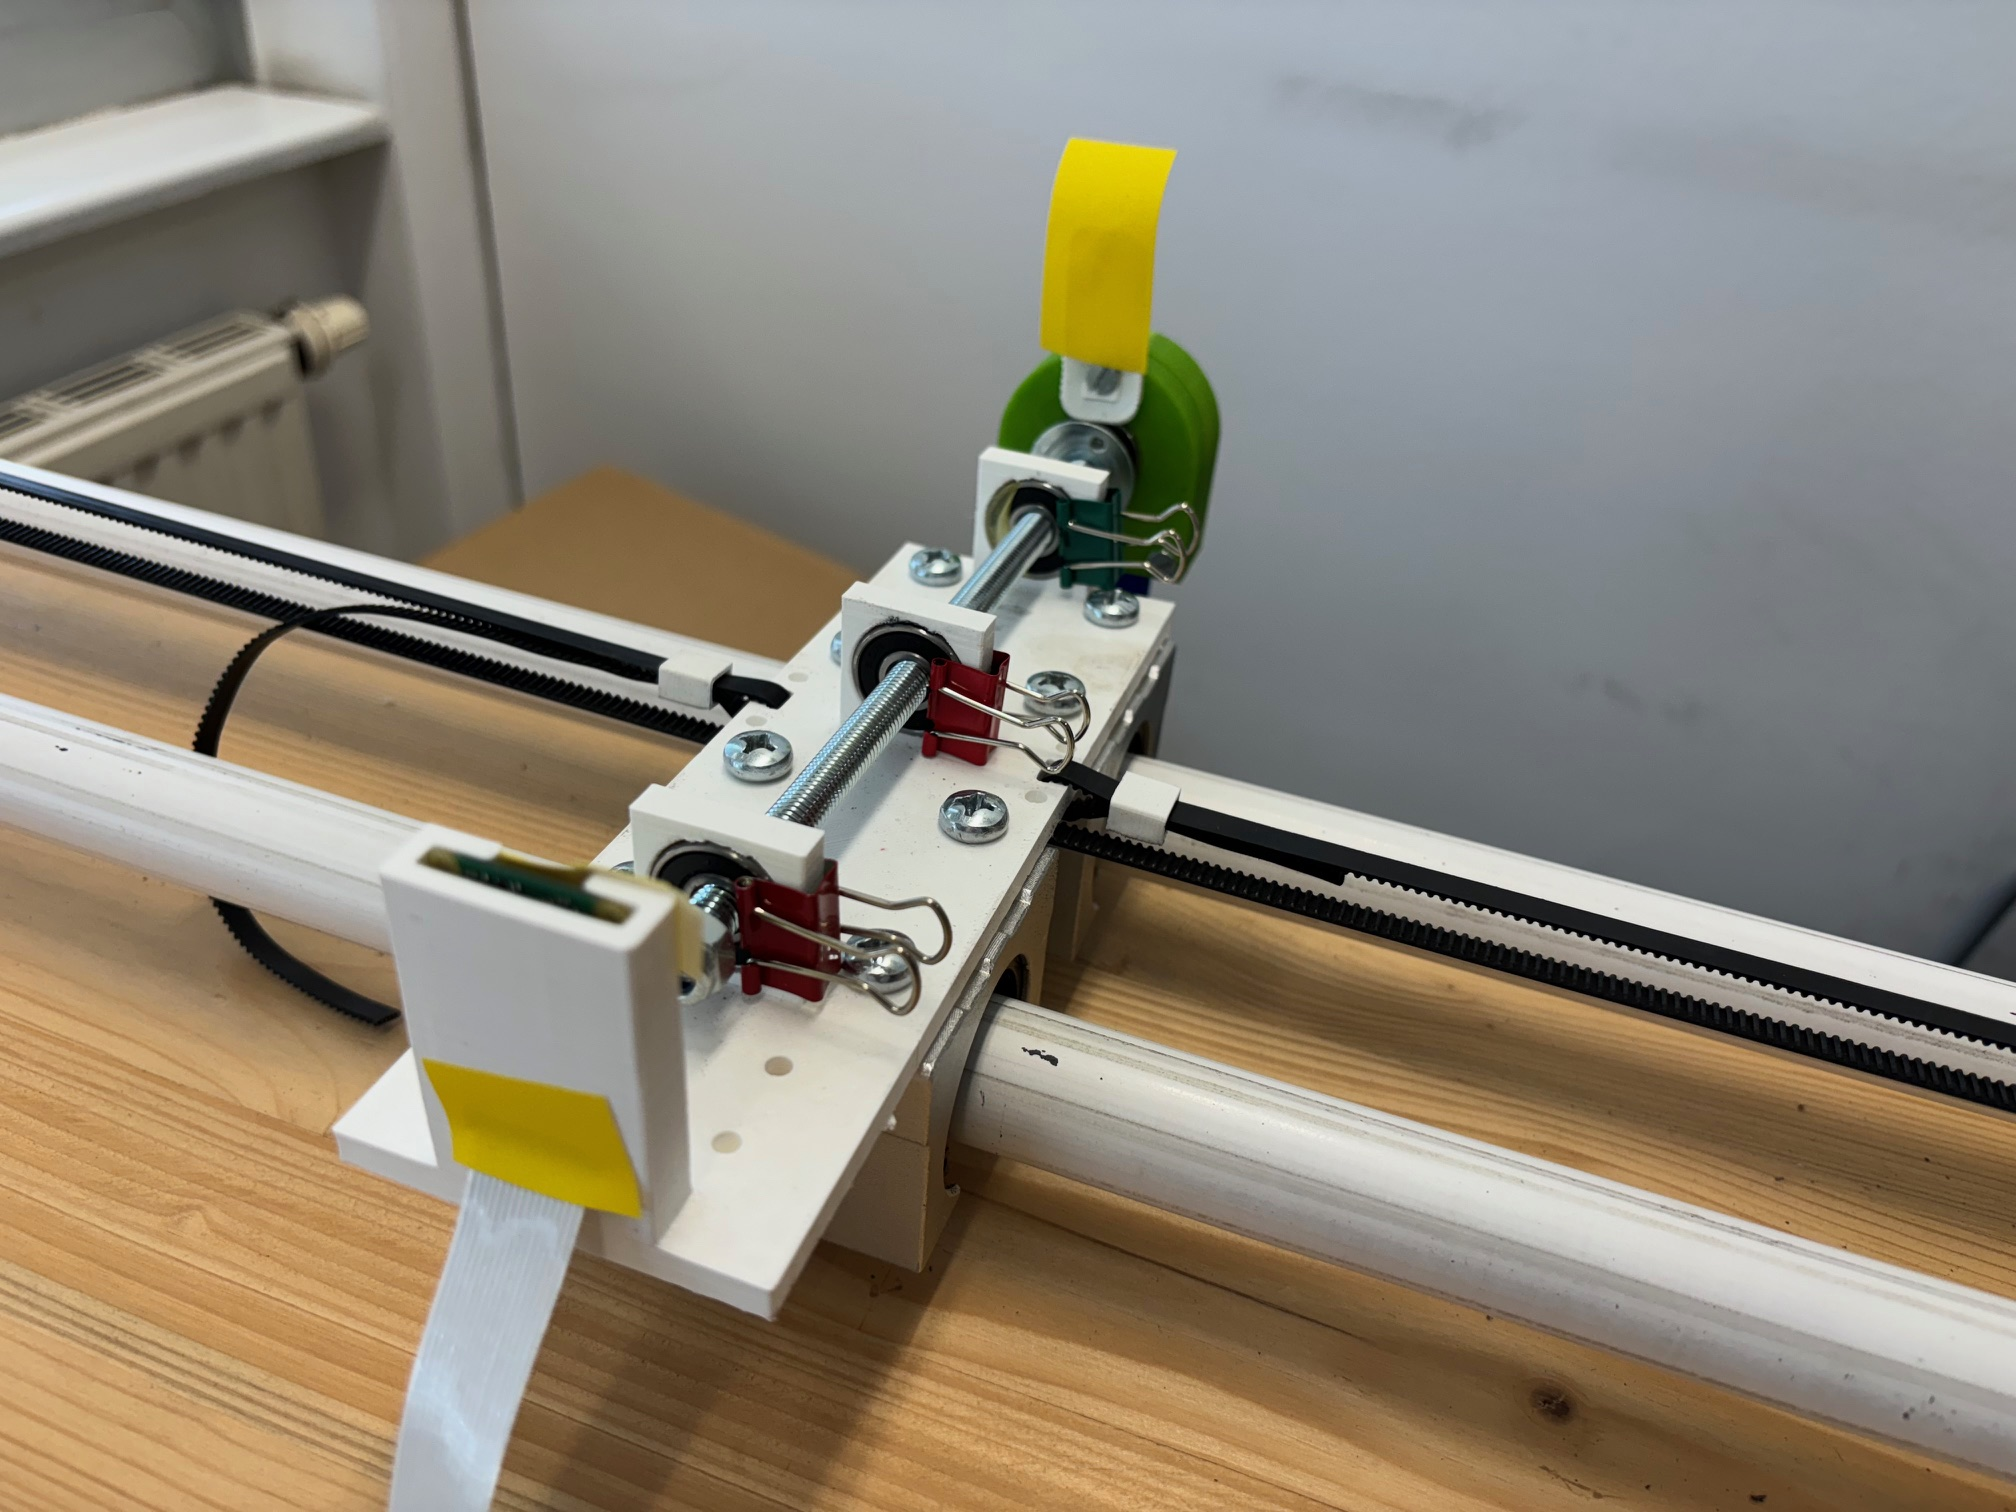
\includegraphics[width=0.8\textwidth]{img/cart.jpg}
    \caption{Cart from 3D printed parts with camera. Clamps are used to fixate moving parts.}
    \label{fig:cart}
\end{figure}
\begin{figure}[htbp]
    \centering
    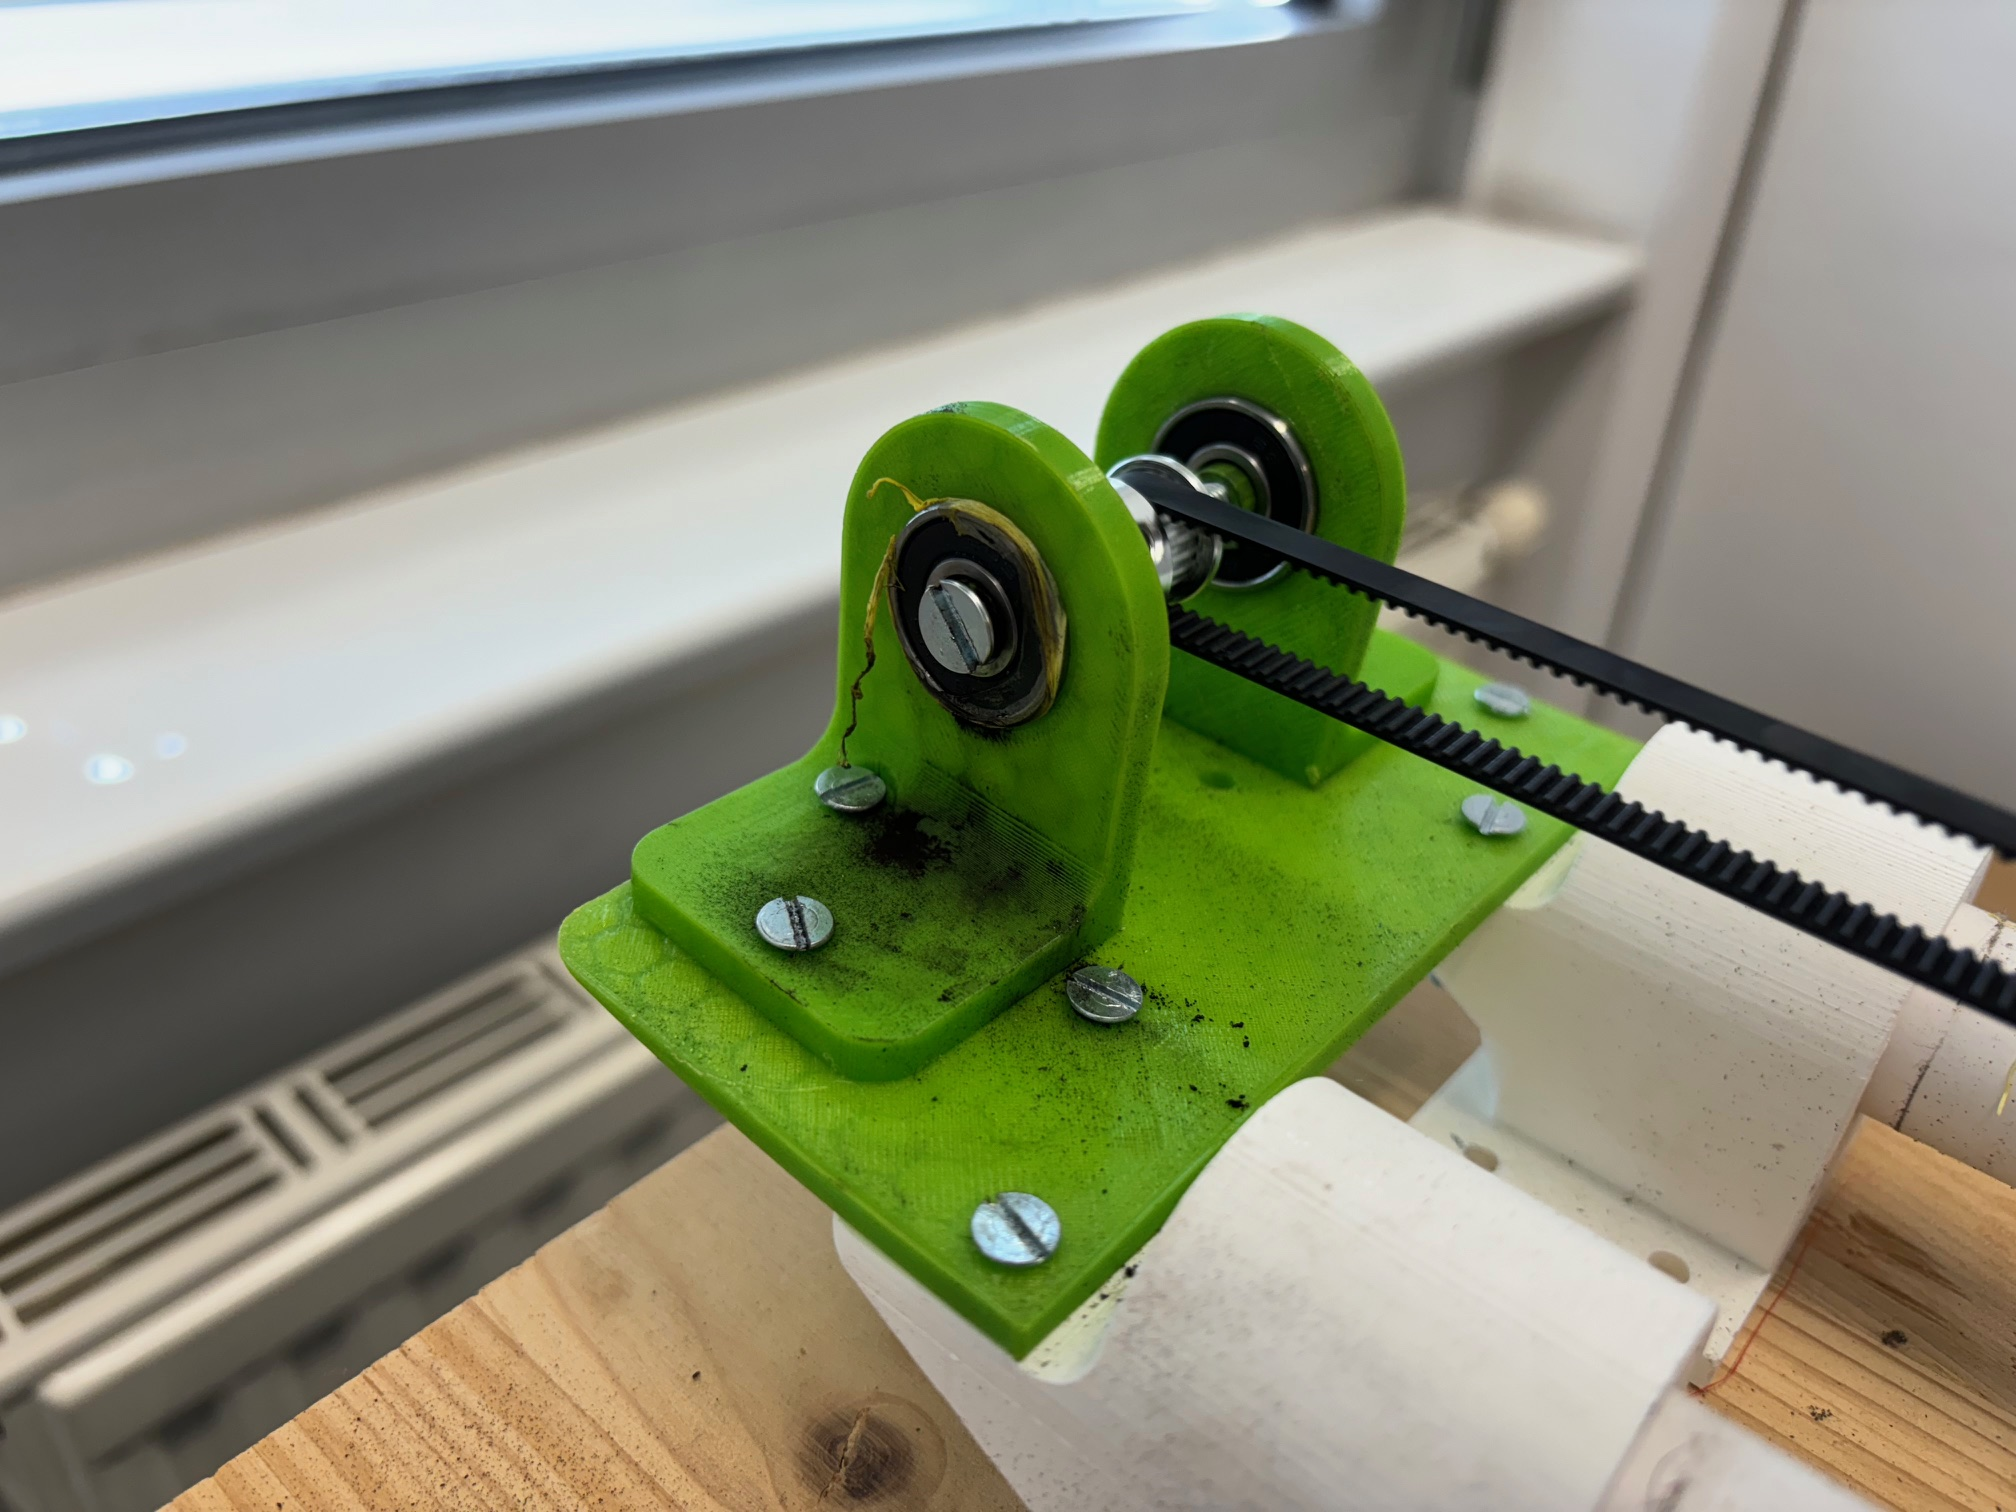
\includegraphics[width=0.8\textwidth]{img/deflection_pulley.jpg}
    \caption{Deflection pulley for the belt}
    \label{fig:deflection_pulley}
\end{figure}
- auf einem Holzbrett im Abstand von 95 cm 2 Halterungen montiert für Metallstangen, auf denen das Cart (\ref{fig:cart}) fahren kann
- auf einer Halterung ist eine Umlenkrolle in Form eines Zahnrades montiert, die den Zahnriemen führt, auf der anderen Halterung ist der Stepper Motor montiert (\ref{fig:deflection_pulley})
- der Zahnriemen muss sehr straff gespannt sein, sonst rutscht er durch und das Cart bewegt sich nicht
- mehrere Halterungen für ein Gewinde, an dem das Pendel hängt
- Pendel ist 3D gedruckt und besteht aus 5 Teilen, die zusammengesteckt werden: 1 blauer breiter Stab und 4 Teile um den Stab, wovon 2 für die Verbindung von Pendel und Gewinde sorgen und 2 für zusätzliches Gewicht am Ende des Pendels sorgen
- ein Stück Plastik mit gelbem Klebeband ist auch am Pendel befestigt, um es der Kamera zu ermöglichen, das Pendel in jeder Position zu erkennen
- insgesamt ist das Pendel 35 cm lang und wiegt 128 g
- eigentlich verlangt das Cart-Pole-Experiment eine reibungslose Oberfläche, auf der das Cart fahren kann, dieses wurde versucht durch Rollen, die um die Metallstangen angebracht sind, zu erreichen, jedoch war die Oberfläche nicht reibungslos genug, sodass das Cart nicht reibungslos fahren konnte. Es ist leider verhältnismäßig viel Kraft notwendig, um das Cart zu bewegen, was die Experimente erschwert hat. Aber laut Escobar et al. (2020) ist das kein Problem, da das Cart-Pole-Experiment auch mit Reibung gelöst werden kann.

\subsection{Stepper Motor}
\begin{figure}[htbp]
    \centering
    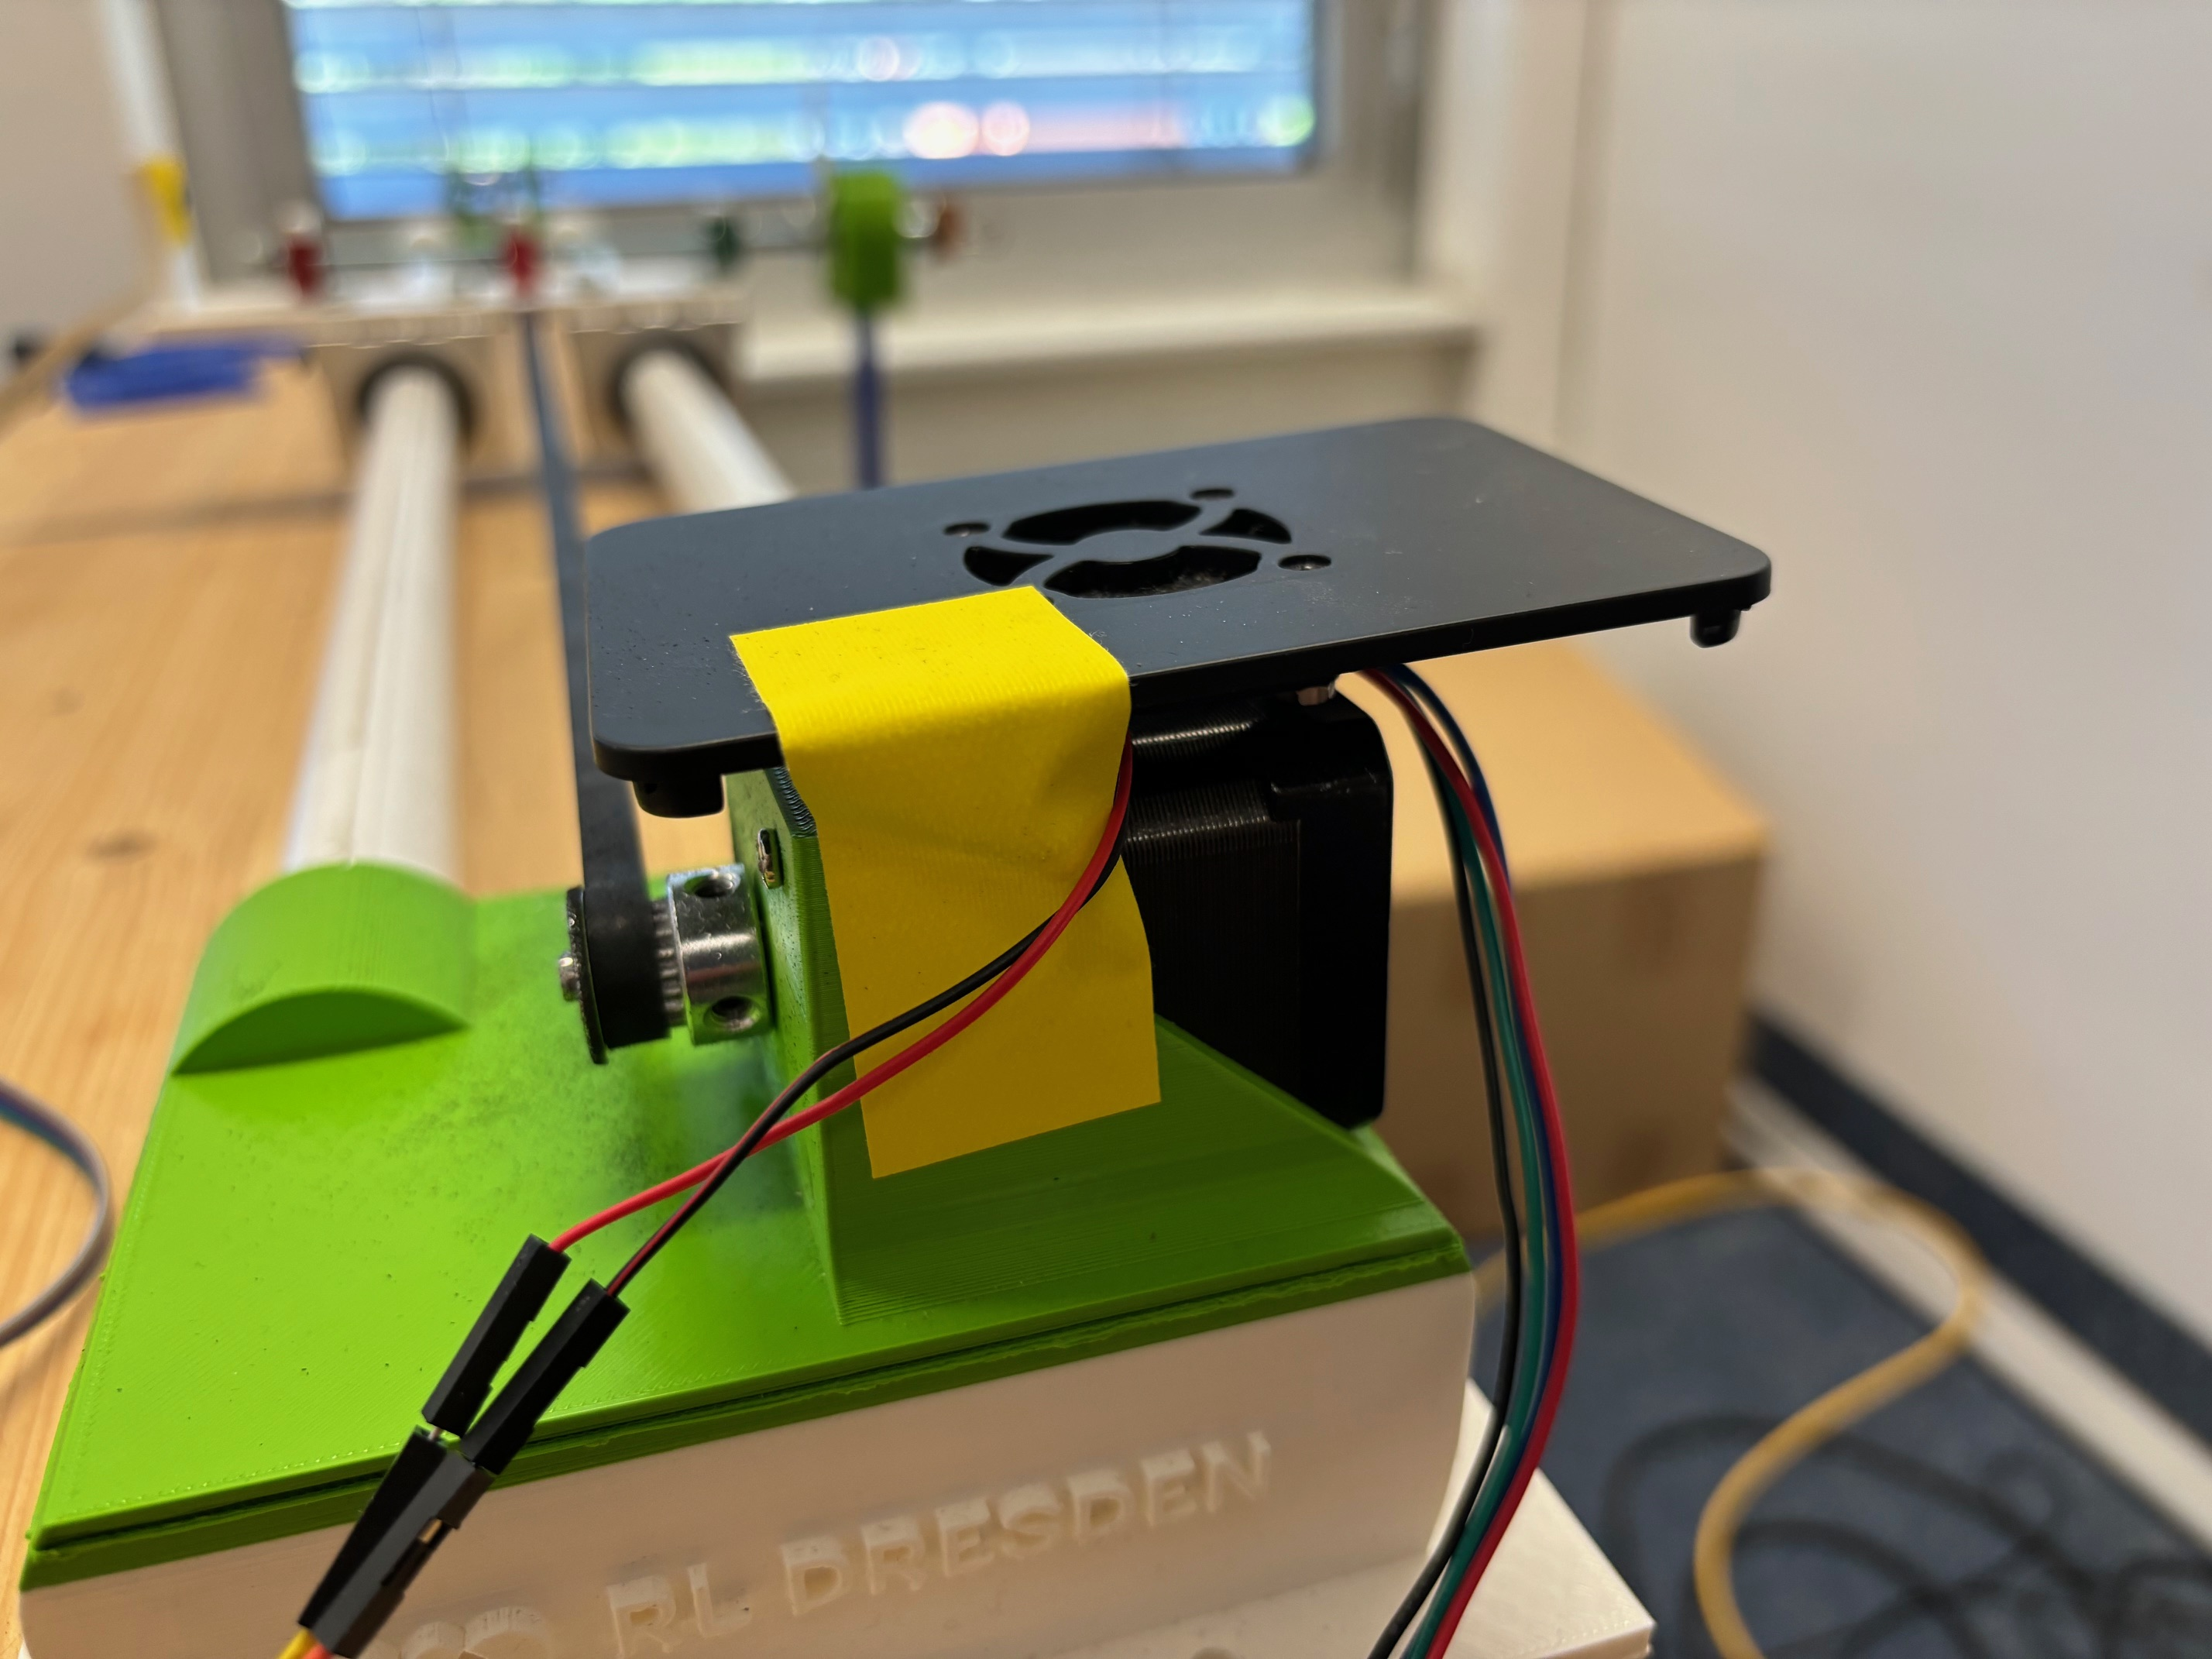
\includegraphics[width=0.8\textwidth]{img/stepper_motor.jpg}
    \caption{Stepper Motor for the Cart}
    \label{fig:stepper_motor}
\end{figure}
- Stepper Motor dreht ein Zahnrand, auf dem sich der Zahnriemen befindet, dadurch wird das Cart bewegt (\ref{fig:stepper_motor})
- bei verschiedenen Experimenten wurden unterschiedliche Stromsträken für den Stepper Motor getestet, der dadurch heiß wurde, deswegen wurde ein Lüfter montiert, der Lüfter ist vom selben Typ wie der Lüfter der einen Raspberry Pi kühlt und wird mit 3.3V betrieben
- verschiedene Stepper Motoren wurden im Verlauf der Experimente probiert, alle vom Typ NEMA 17, 1 Motor mit der Bezeichnung MOT-AN-S-060-005-042-L-A-AAAA von igus, 2 Motoren mit der Bezeichnung 17HS19-2004S1 von stepperonline, wovon einer nicht akkurat war
- der Motor von igus verträgt eine Stromstärke von 1.8A, die anderen Motoren vertragen 2A
- die Stromstärke wurde im Verlauf der Experimente verändert, um die beste Leistung zu erzielen, ohne den Motor zu überhitzen

\subsection{Stepper Motor Control}
- alle Motoren wurden mit einem Makeblock 2H Microstep Driver angesteuert, der mit einem Arduino verbunden ist
- der Arduino ist mit einem Raspberry Pi und Microusb verbunden
- alle Stepper Motoren wurden mit einer Schrittwinkelauflösung von 1.8$^\circ$ betrieben (12800 Schritte pro Umdrehung)

\subsection{Camera}
\begin{figure}[htbp]
    \centering
    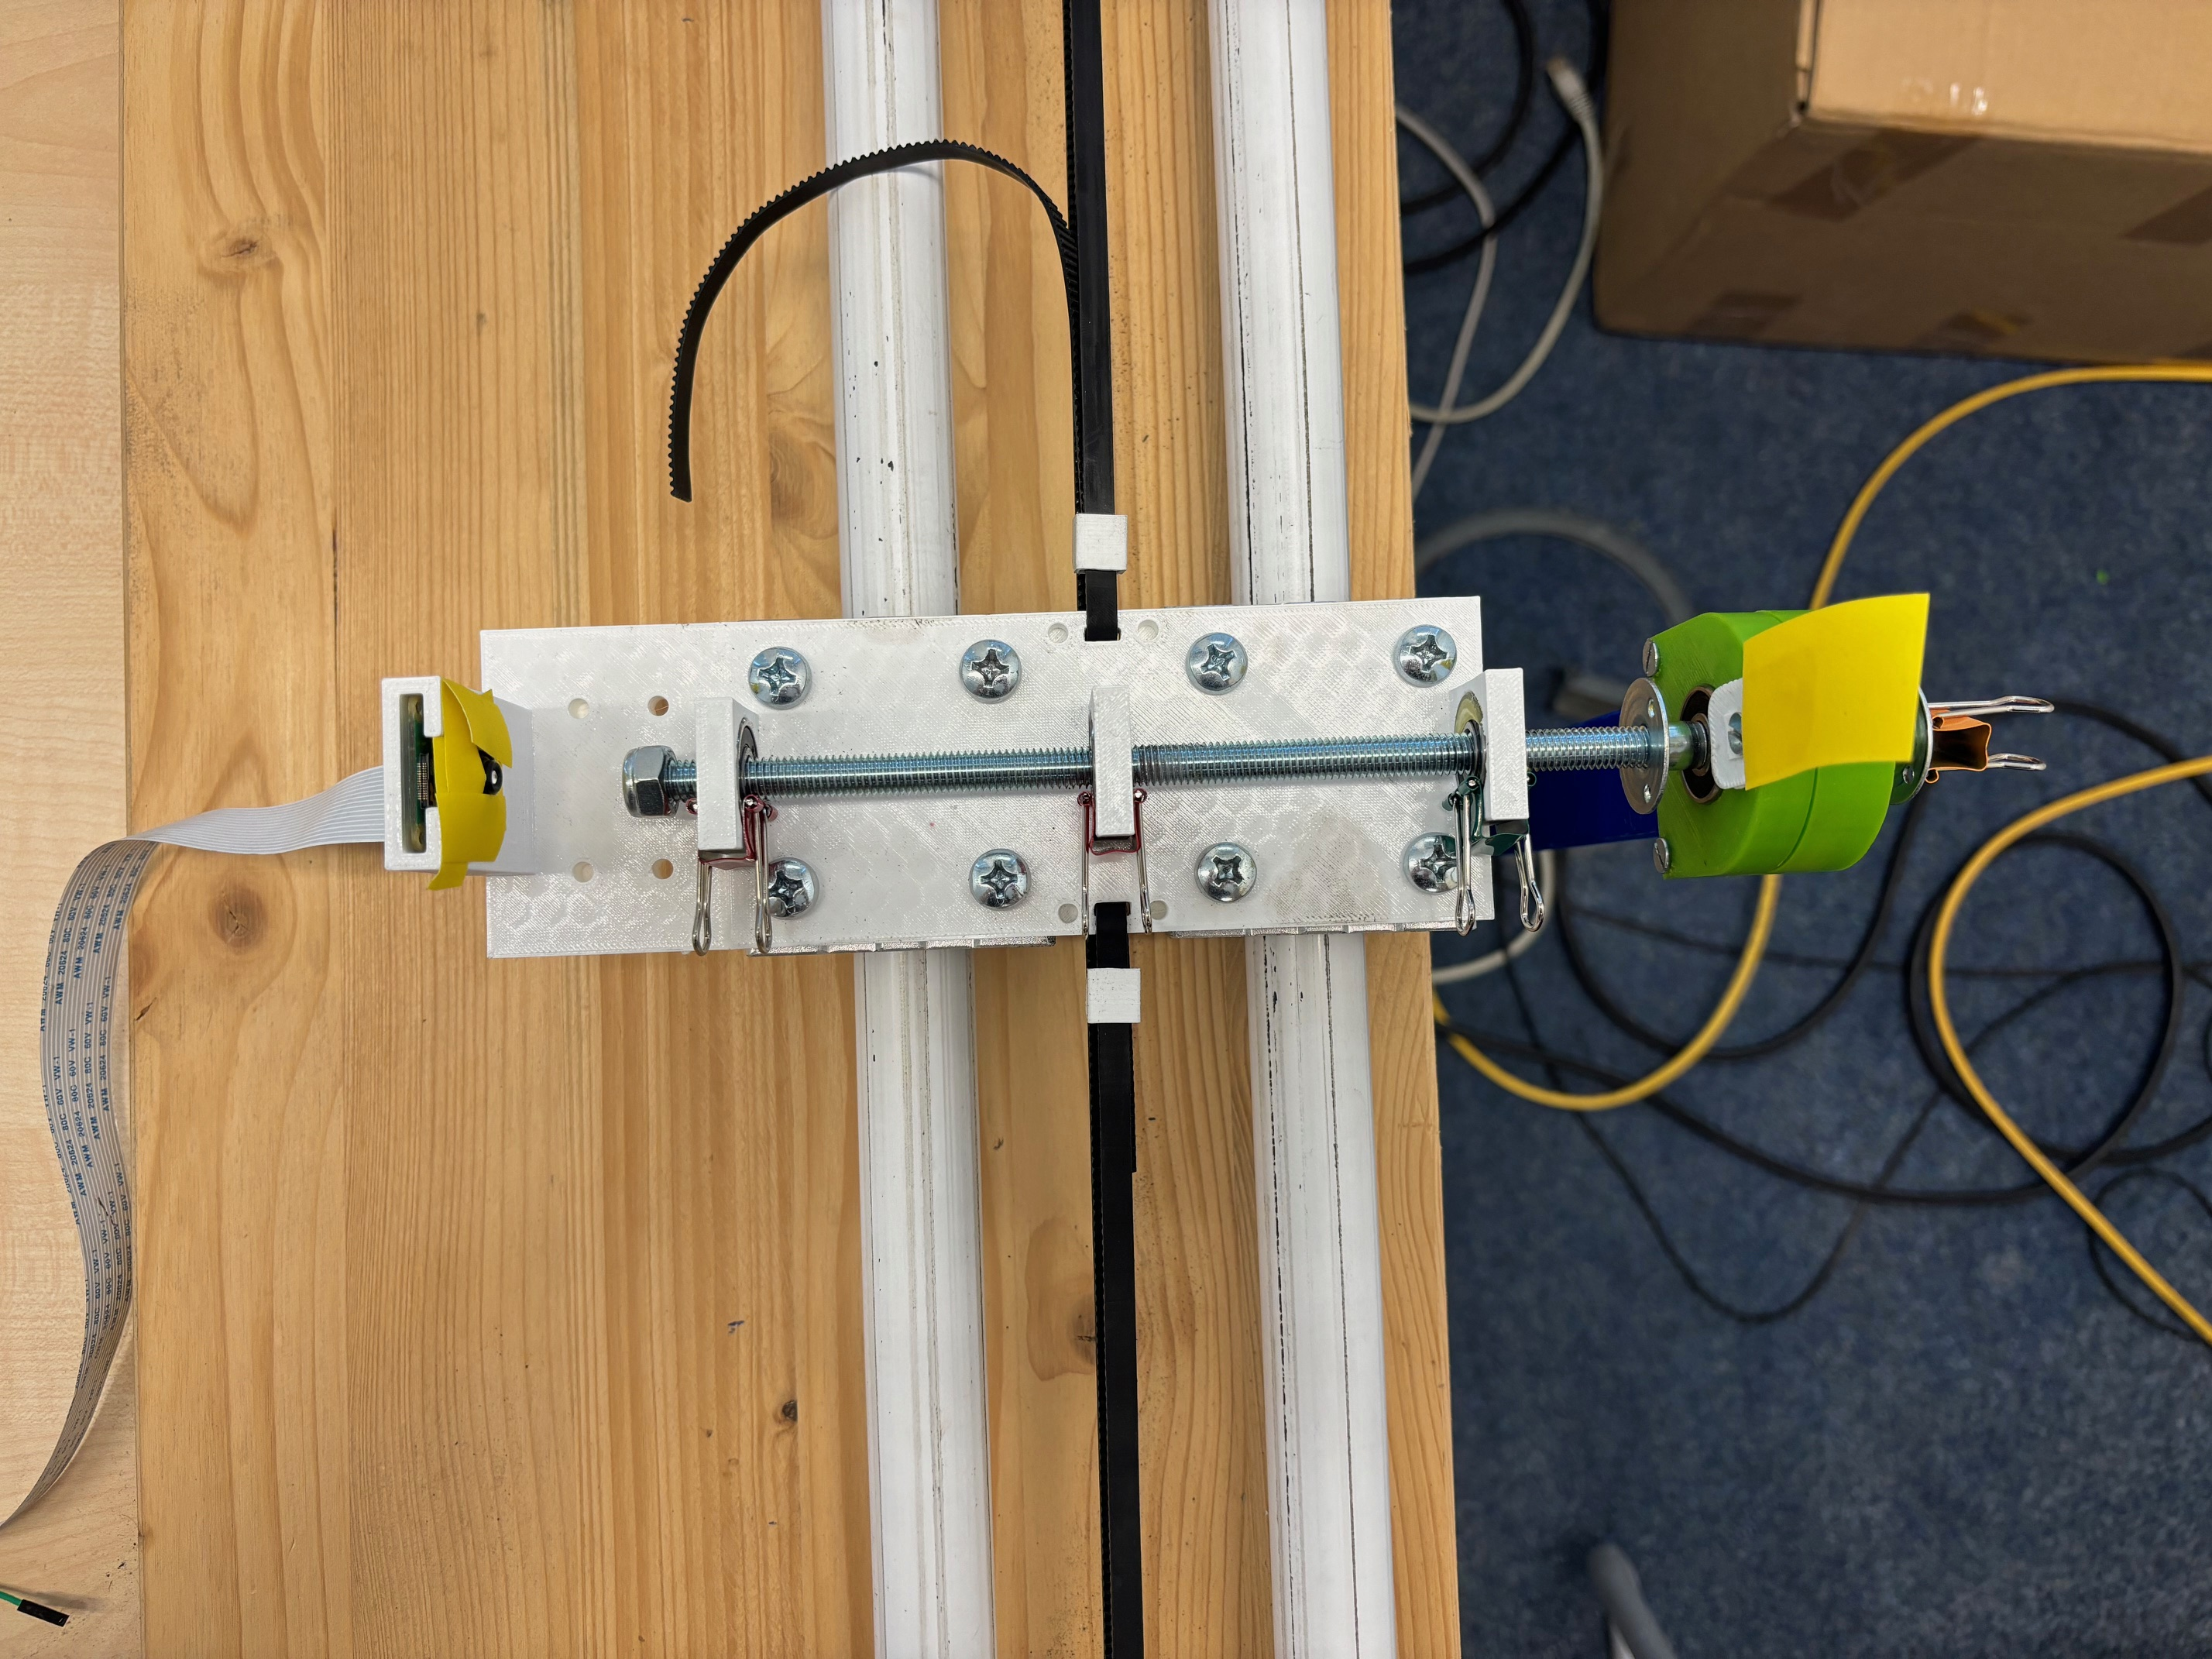
\includegraphics[width=0.8\textwidth]{img/camera.jpg}
    \caption{Camera to detect the angle of the pendulum}
    \label{fig:camera}
\end{figure}
- Kamera ist eine Picam, die in einem 3D gedruckten Gehäuse montiert ist, das an dem Cart befestigt ist (\ref{fig:camera})
- Kamera ist mit einem Raspberry Pi verbunden, der die Bilder der Kamera verarbeitet
- Position der Kamera darf sich nicht verändern, da sonst die Winkel des Pendels, die erkannt werden sollen, nicht mehr korrekt sind
- Deaktivieren des Autofocus der Kamera, um die Bilder schneller zu machen und immer die gleiche Schärfe zu haben
- Einsatz von Klebeband, um die Kamera zu fixieren

\section{Software Architecture}
\subsection{Reinforcement Learning Agent}
- Entwicklung einer eigenen Environment auf Basis von OpenAI Gym, die die Cart-Pole-Umgebung nachbildet
- wichtigste Änderung: Überschreiben der step-Funktion, damit die ausgewählten Aktionen in Nachrichten umgewandelt werden, die an den Arduino gesendet werden, um das Cart zu bewegen
- Algorithmus: PPO, Implementierung von stable baselines 3
- Verarbeitung der Bilder der Kamera in einem eigenen Skript, welches unabhängig vom Reinforcement Learning Agent läuft, um die Winkel des Pendels zu bestimmen
- Winkel starten bei 0 in der oberen Position und gehen bis 180 Grad in der unteren Position, auf der linken Seite des Pendels von 0 bis 180 Grad, auf der rechten Seite von 0 bis -180 Grad
- Senden der Winkel und weiterer Informationen über ZeroMQs Implementeriung eines TCP Sockets an den Reinforcement Learning Agent
- Vorteil: bessere Nutzung der 4 Kerne des Raspberry Pis (1 Kern für RL Agent, 1 Kern für Bildverarbeitung), Bilder können häufiger gemacht werden, akuratere Bestimmung der Winkelgeschwidigkeit durch mehr Messungen, Reduktion des Delays in den Entscheidungen des RL Agents, da die Bilder nicht mehr verarbeitet werden müssen, bevor der RL Agent eine Aktion auswählt

\subsection{Control Algorithms}
- Kommunikation des Raspberry Pi mit dem Arduino über USB als serielle Schnittstellenverbindung
- eigenes Protokoll, Nachrichten werden in Form von Strings übertragen, Strings haben die Form "<letter,number>", die Buchstaben stehen für die Art der Nachricht, die Zahlen für die Werte
\begin{table}
    \caption{Types of messages for the Arduino}
    \label{tab:types_of_messages}
    \begin{tabular}{|c|c|}
        \hline
        Type & Description \\
        \hline
        v & Set the speed in steps per second \\
        a & Set the acceleration in steps per second$^2$ \\
        m & Move the stepper motor to a certain position \\
        r & Move the stepper motor relative to its current position \\
        h & Set the current position as home position. Value is always 0 \\
        s & Set the steps per revolution \\
        p & Get the current position. Value is always 0 \\
        \hline
    \end{tabular}
    \end{table}
- Arduino kennt immer die aktuelle Position durch mitzählen der durchgeführten Schritte und stoppt den Motor automatisch, wenn das Cart das Ende der Stangen erreicht. Dafür ist es notwendig, den Home-Punkt immer in der Mitte des Streckenabschnitts zu setzen, den das Cart zurücklegen soll, um sicherzustellen, dass das Cart immer anhält, wenn es das Ende der Stange erreicht, die maximale Anzahl der Umdrehungen des Stepper Motors bevor das Cart das Ende der Stangen erreicht, wurde mit 9 ermittelt.
- Der Raspberry Pi sendet die Nachrichten an den Arduino, um das Cart zu bewegen, und durch die Asynchronität des Systems kann der Raspberry Pi in der Zwischenzeit andere Berechnungen durchführen, um die nächste Aktion des Reinforcement Learning Agents zu bestimmen, während das Cart sich bewegt
- Der Ardoino führt (bei Angabe einer Geschwindigkeit) die Bewegung des Carts solange aus, bis er eine neue Nachricht bekommt oder das Cart das Ende der Stange erreicht hat

- weiterhin wurde eine funktion eingebaut, die ermittelt, ob das Büro leer ist, um diese Mitarbeiter nicht durch die Geräusche zu stören, die das Cart macht, wenn es sich bewegt
- ob das Büro leer ist, hängt aktuell nur von der Zeit ab, aktuell wird davon ausgegangen, dass das Büro von 8:30 am Morgen bis 18:30 am Abend von Montag bis Freitag besetzt ist. Außerhalb dieser Zeiten wird davon ausgegangen, dass das Büro leer ist und das Cart sich bewegen kann ohne jemanden zu stören.
- Die Überprüfung, ob das Büro leer ist, wird bei jedem reset des RL Agents durchgeführt (Aufruf der reset-Funktion der Gym Environment). Ist das Büro nicht leer, so wird 10 Minuten gewartet, bis erneut geprüft wird.
